\documentclass[a4paper,14pt, unknownkeysallowed]{extreport}

\usepackage{cmap} % Улучшенный поиск русских слов в полученном pdf-файле
\usepackage[T2A]{fontenc} % Поддержка русских букв
\usepackage[utf8]{inputenc} % Кодировка utf8
\usepackage[english,russian]{babel} % Языки: русский, английский
\usepackage{enumitem}


\usepackage{threeparttable}

\usepackage[14pt]{extsizes}

\usepackage{caption}
\captionsetup{labelsep=endash}
\captionsetup[figure]{name={Рисунок}}

% \usepackage{ctable}
% \captionsetup[table]{justification=raggedleft,singlelinecheck=off}

\usepackage{amsmath}

\usepackage{geometry}
\geometry{left=30mm}
\geometry{right=15mm}
\geometry{top=20mm}
\geometry{bottom=20mm}

\usepackage{titlesec}
\titleformat{\section}
	{\normalsize\bfseries}
	{\thesection}
	{1em}{}
\titlespacing*{\chapter}{0pt}{-30pt}{8pt}
\titlespacing*{\section}{\parindent}{*4}{*4}
\titlespacing*{\subsection}{\parindent}{*4}{*4}

\usepackage{setspace}
\onehalfspacing % Полуторный интервал

\frenchspacing
\usepackage{indentfirst} % Красная строка
\setlength{\parindent}{1.25cm}

\usepackage{titlesec}
\titleformat{\chapter}{\LARGE\bfseries}{\thechapter}{20pt}{\LARGE\bfseries}
\titleformat{\section}{\Large\bfseries}{\thesection}{20pt}{\Large\bfseries}

\usepackage{multirow}
\usepackage{listings}
\usepackage{xcolor}

% Для листинга кода:
\lstset{ %
language=caml,                 % выбор языка для подсветки (здесь это С)
basicstyle=\small\sffamily, % размер и начертание шрифта для подсветки кода
numbers=left,               % где поставить нумерацию строк (слева\справа)
stepnumber=1,                   % размер шага между двумя номерами строк
numbersep=5pt,                % как далеко отстоят номера строк от подсвечиваемого кода
showspaces=false,            % показывать или нет пробелы специальными отступами
showstringspaces=false,      % показывать или нет пробелы в строках
showtabs=false,             % показывать или нет табуляцию в строках
frame=single,              % рисовать рамку вокруг кода
tabsize=2,                 % размер табуляции по умолчанию равен 2 пробелам
captionpos=t,              % позиция заголовка вверху [t] или внизу [b] 
breaklines=true,           % автоматически переносить строки (да\нет)
breakatwhitespace=false, % переносить строки только если есть пробел
escapeinside={\#*}{*)}   % если нужно добавить комментарии в коде
}



% plot
\usepackage{graphicx}
\usepackage{pgfplots}
\usepackage{filecontents}
\usetikzlibrary{datavisualization}
\usetikzlibrary{datavisualization.formats.functions}

\graphicspath{ {img/} }


\usepackage{subcaption}

\captionsetup{labelsep=endash}
\captionsetup[figure]{name={Рисунок}}



\usepackage[justification=centering]{caption} % Настройка подписей float объектов

\usepackage[unicode,pdftex]{hyperref} % Ссылки в pdf
\hypersetup{hidelinks}

\usepackage{csvsimple}

\newcommand{\code}[1]{\texttt{#1}}

\begin{document}
	
\begin{titlepage}
	\newgeometry{pdftex, left=2cm, right=2cm, top=2.5cm, bottom=2.5cm}
	\fontsize{12pt}{12pt}\selectfont
	\noindent \begin{minipage}{0.15\textwidth}
		
\includegraphics[width=\linewidth]{img/main_logo.jpg}
	\end{minipage}
	\noindent\begin{minipage}{0.9\textwidth}\centering
		\textbf{Министерство науки и высшего образования Российской Федерации}\\
		\textbf{Федеральное государственное бюджетное образовательное учреждение высшего образования}\\
		\textbf{«Московский государственный технический университет имени \newline Н. Э. Баумана}\\
		\textbf{(национальный исследовательский университет)»}\\
		\textbf{(МГТУ им. Н. Э.~Баумана)}
	\end{minipage}
	
	\noindent\rule{18cm}{3pt}
	\newline\newline
	\noindent ФАКУЛЬТЕТ $\underline{\text{«Информатика и системы управления»~~~~~~~~~~~~~~~~~~~~~~~~~~~~~~~~~~~~~~~~~~~~~~~~~~~~~~~}}$ \newline\newline
	\noindent КАФЕДРА $\underline{\text{«Программное обеспечение ЭВМ и информационные технологии»~~~~~~~~~~~~~~~~~~~~~~~}}$\newline\newline\newline\newline\newline\newline\newline
	
	
	\begin{center}
		\noindent\begin{minipage}{1.3\textwidth}\centering
		\Large\textbf{   ~~~ Лабораторная работа №1}\newline
		\textbf{по дисциплине "Анализ Алгоритмов"}\newline\newline\newline
		\end{minipage}
	\end{center}
	
	\noindent\textbf{Тема} 			$\underline{\text{Расстояние Левенштейна и Дамерау-Левенштейна}}$\newline\newline
	\noindent\textbf{Студент} 		$\underline{\text{Светличная А.А.}}$\newline\newline
	\noindent\textbf{Группа} 		$\underline{\text{ИУ7-53Б}}$\newline\newline
	\noindent\textbf{Преподаватель} $\underline{\text{Волкова Л. Л., Строганов Ю.В.}}$\newline
	
	\begin{center}
		\vfill
		Москва~---~\the\year
		~г.
	\end{center}
	\restoregeometry
\end{titlepage}
	
	\setcounter{page}{2}
	\tableofcontents
	
	\newpage
	\chapter*{Введение}
	
	\addcontentsline{toc}{chapter}{Введение}
	
В программировании большое количество задач связано с обработкой строк. 
В данной рабораторной работе будут рассмотрены алгоритмы, использующие расстояние Левенштейна ~--~ метрика, позволяющая определить «схожесть» двух строк, вычисляя минимальное количество операций вставки, удаления, замены одного символа на другой, необходимых для превращения одной строки в другую.

Расстояние Левенштейна применяется в теории информации и компьютерной лингвистике для:

\begin{itemize}
	\item[1)] исправления ошибок в слове;
	\item[2)] сравнения текстовых файлов утилитой diff;
	\item[3)] для сравнения генов, хромосом и белков в биоинформатике.
\end{itemize}

	
\chapter{Аналитическая часть}
	
\section{Цель и задачи}
	
Целью данной работой является получение навыка динамического программирования на примере разработки алгоритмов поиска редакционных расстояний. 
    
Для достижения поставленной цели требуется решить следующие задачи:
    
\begin{itemize}
    \item[1)] изучить расстояния Левенштейна и Дамерау-Левенштейна;
    \item[2)] разработать указнные алгоритмы поиска расстояний;
    \item[3)] реализовать разработанные алгоритмы;
    \item[4)] провести сравнительный анализ реализаций алгоритмов по затраченному процессорному времени и памяти на основе экспериментальных данных;
    \item[5)] описать и обосновать полученные результаты в отчете о выполненной лабораторной работе.
\end{itemize}
	
	
\section{Итерационный алгоритм поиска расстояния Левенштейна}

Расстояние Левенштейна [1] ~--~ это минимальное количество операций вставки, удаления и замены, необходимох для превращения одной строки в другую.

Цены операций могут зависеть от вида операций (вставка, удаление, замена) и/или от участвующих в ней символов, отражая разную вероятность разных ошибок при вводе текста и т.п. В общем случае

\begin{itemize}
	\item[1)] $w(a, b)$ ~--~ цена замены символа $a$ на $b$, R (от англ. replace);
	\item[2)] $w(\lambda, b)$ ~--~ цена вставки символа $b$, I (от англ. insert);
	\item[3)] $w(a, \lambda)$ ~--~ цена удаления символа $a$, D (от англ. delete).
\end{itemize}

Для решения задачи о редакционном расстоянии необходимо найти последовательность замен, минимизирующую суммарную цену. 
Расстояние Левенштейна является частным случаем этой задачи при

\begin{itemize}
	\item[1)] $w(a, a) = 0$;
	\item[2)] $w(a, b) = 1$, $a \neq b$;
	\item[3)] $w(\lambda, b) = 1$;
	\item[4)] $w(a, \lambda) = 1$.
\end{itemize}

Имеется две строки $S_{1}$ и $S_{2}$, длинной m и n соответственно. 
Расстояние Левенштейна рассчитывается по рекуррентной формуле (\ref{eq:L}).

\begin{equation}
	\label{eq:L}
	D(i, j) = \begin{cases}
	0, &\text{i = 0, j = 0}\\
	i, &\text{j = 0, i > 0}\\
	j, &\text{i = 0, j > 0}\\
	min \begin{cases}
		D(i, j - 1) + 1\\
		D(i - 1, j) + 1\\
		D(i - 1, j - 1) + \begin{cases}
                        		0, &\text{если $S_{i}$ = $S_{j}$,}\\
                        		1, &\text{иначе}
                        	\end{cases}\\\\
	\end{cases}
	&\text{i > 0, j > 0}
	\end{cases}
\end{equation}

\section{Итерационный алгоритм поиска расстояния Дамерау-Левенштейна}

В алгоритме поиска расстояния Дамерау-Левенштейна, помимо вставки, удаления, и замены присутствует  еще одна редакторская операция - транспозиция T (от англ. transposition).

Расстояние Дамерау-Левенштейна может быть вычисленно по рекуррентной формуле (\ref{eq:DL}).

\begin{equation}
	\label{eq:DL}
	D(i, j) = \begin{cases}
		
		0, &\text{i = 0, j = 0,}\\
		i, &\text{j = 0, i > 0,}\\
		j, &\text{i = 0, j > 0,}\\
		
		\min \lbrace \\
		\qquad D(i, j-1) + 1,&\text{i > 0, j > 0,}\\
		\qquad D(i-1, j) + 1,&\text{$S_{i}$ = $S_{j-1}$,}\\
		\qquad D(i-2, j-2) + 1,&\text{$S_{i-1}$ = $S_{j}$,}\\
		\qquad D(i-1, j-1) + \begin{cases}
                        		0, &\text{если $S_{i}$ = $S_{j}$,}\\
                        		1, &\text{иначе}
                        	\end{cases}\\
		\rbrace,\\
		
		\min \lbrace \\
		\qquad D(i, j-1) + 1,\\
		\qquad D(i-1, j) + 1,&\text{иначе}\\
		\qquad D(i-1, j-1) + \begin{cases}
                        		0, &\text{если $S_{i}$ = $S_{j}$,}\\
                        		1, &\text{иначе}
                        	\end{cases}\\
		\rbrace
	\end{cases}
\end{equation}
	
\section{Рекурсивный алгоритм поиска расстояния Дамерау-Левенштейна}
	
Рекурсивный алгоритм нахождения расстояния Дамерау-Левенштейна отличается от его итерационной версии тем, что в нем вместо использования матрицы для хранения предыдущих значений, необходимых для подсчета последующих, эти значения вычисляются каждый раз рекурсивно. 
	
\section{Рекурсивный алгоритм поиска расстояния Дамерау-Левенштейна с использованием кеша}
Данный алгоритм является оптимизацией рекурсивного алгоритма нахождения расстояния Дамерау-Левенштейна. 
Оптимизация заключается в использовании кеша, который представляется собой матрицу, в которую записываются значения, вычисленные на шагах рекурсии. 
Таким образом, при необходимости вычисления какого-либо нового значения по реккурентной формуле, величины, необходимые для этого не вычисляются каждый раз: сначала проверяется, было ли уже вычислено данное значения, и только лишь в случае, если этого не происходило, выполняются рекурсивные вычисления для его получения.
	
	
\section*{Вывод}
	
В данном разделе были рассмотрены алгоритмы нахождения расстояния Левенштейна и Дамерау-Левенштейна, формулы которых задаются реккурентно, а следовательно, данные алгоритмы могут быть реализованы рекурсивно и итерационно.
	
\clearpage
	
\chapter{Конструкторская часть}
	
\section{Описание типов данных}
	
Для реализации алгоритмов Левенштейна и Дамерау-Левенштейна были использованы следующие типы данных:

\begin{enumerate}
    \item[1)] строка - массив типа $char$;
    \item[2)] длина строки - число типа $int$;
    \item[3)] матрица - структура, содержащая двумерный массив типа $int$ и размерности типа $int$.
\end{enumerate}
	
\section{Оценка затрат алгоритмов по памяти}
	
Алгоритмы Левенштейна и Дамерау-Левенштейна не отличаются по использованию памяти, поэтому достаточно рассмотреть итеррационную и рекурсивную реализации одного алгоритма.

Затраты по памяти для итерационного алгоритм поиска расстояния Левенштайна (Дамерау-Левенштейна):

	\begin{enumerate}
	\item[1)] длины строк n, m -- $2 \cdot sizeof(int)$;
	\item[2)] матрица -- $(n + 1) \cdot (m + 1) \cdot sizeof(int) + 2 \cdot sizeof(int)$;
	\item[3)] строки -- $(n + m + 2) \cdot sizeof(char)$;
	\item[4)] дополнительные переменные (i, j, res, offset) -- $4 \cdot sizeof(int)$; 
	\item[5)] адрес возврата.
	\end{enumerate}
	
	Суммарные затраты по памяти:
	
	$(n + 1) \cdot (m + 1) \cdot sizeof(int) + 7 \cdot sizeof(int) + (n + m + 2) \cdot sizeof(char)$\newline

    \clearpage
    
	Затраты по памяти для рекурсивного алгоритма поиска расстояния Дамерау-Левенштейна для одного вызова:
	
	\begin{enumerate}
	\item[1)] длины строк n, m -- $2 \cdot sizeof(int)$;
	\item[2)] строки -- $(n + m + 2) \cdot sizeof(char)$;
	\item[3)] дополнительные переменные (res, offset) -- $2 \cdot sizeof(int)$; 
	\item[4)] адрес возврата.
	\end{enumerate}
	
	Суммарные затраты по памяти (R -- количество вызовов рекурсии):
	
	$(4 \cdot sizeof(int) + (n + m + 2) \cdot sizeof(char)) \cdot R$\newline
	
	Затраты по памяти для рекурсивного алгоритма поиска расстояния Дамерау-Левенштейна с кешем для одного вызова:
	
	\begin{enumerate}
	\item[1)] длины строк n, m -- $2 \cdot sizeof(int)$;
	\item[2)] строки -- $(n + m + 2) \cdot sizeof(char)$;
	\item[3)] дополнительные переменные (res, offset) -- $2 \cdot sizeof(int)$; 
	\item[4)] матрица -- $(n + 1) \cdot (m + 1) \cdot sizeof(int) + 2 \cdot sizeof(int)$;
	\item[5)] адрес возврата.
	\end{enumerate}
	
	Суммарные затраты по памяти (R -- количество вызовов рекурсии):
	
	$(6 \cdot sizeof(int) + (n + m + 2) \cdot sizeof(char)) \cdot R + (n + 1) \cdot (m + 1) \cdot sizeof(int)$\newline
	
	\section{Описания алгоритмов}
	
	На рисунках ниже показаны схемы алгоритмов Левенштейна и Дамерау-Левен\-штейна.
	
	\begin{figure}
		\centering
		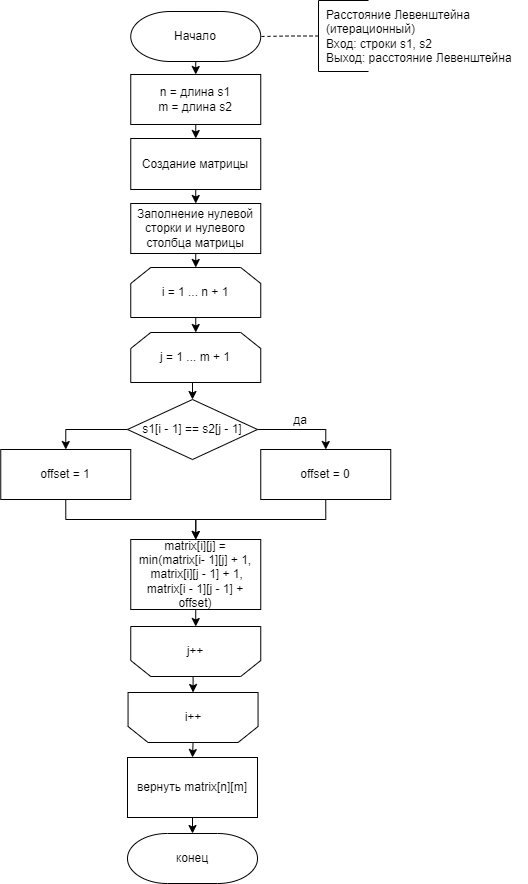
\includegraphics[width=0.8\linewidth]{Lev}
		\caption{Схема итерационного алгоритма поиска расстояния Левенштейна}
		\label{fig:schema_bucket_1}
	\end{figure}
	
	\begin{figure}
		\centering
		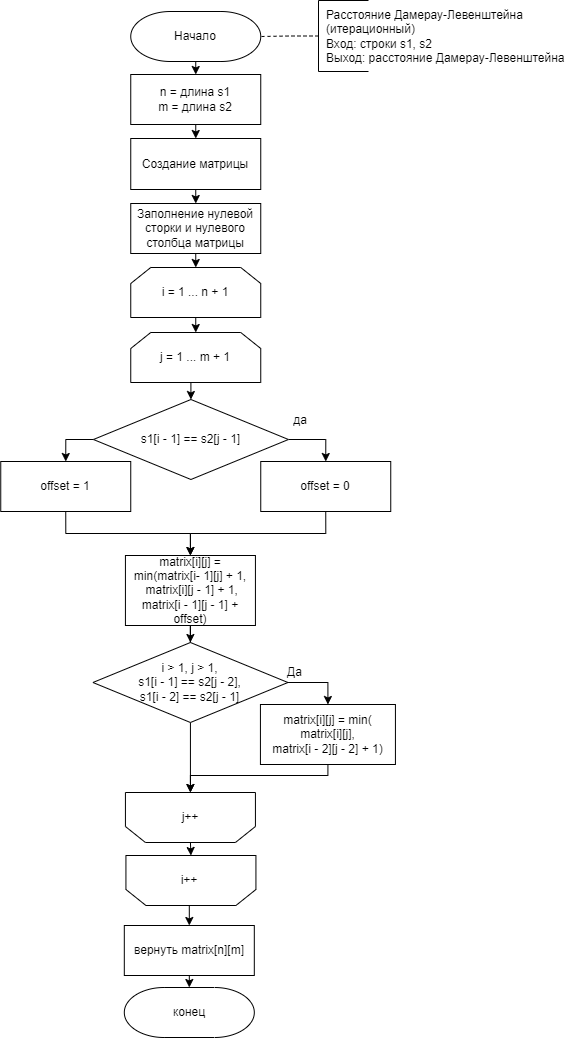
\includegraphics[width=0.7\linewidth]{DamLev}
		\caption{Схема итерационного алгоритма поиска расстояния Дамерау-Левенштейна}
		\label{fig:schema_bucket_2}
	\end{figure}
	
	\begin{figure}
		\centering
		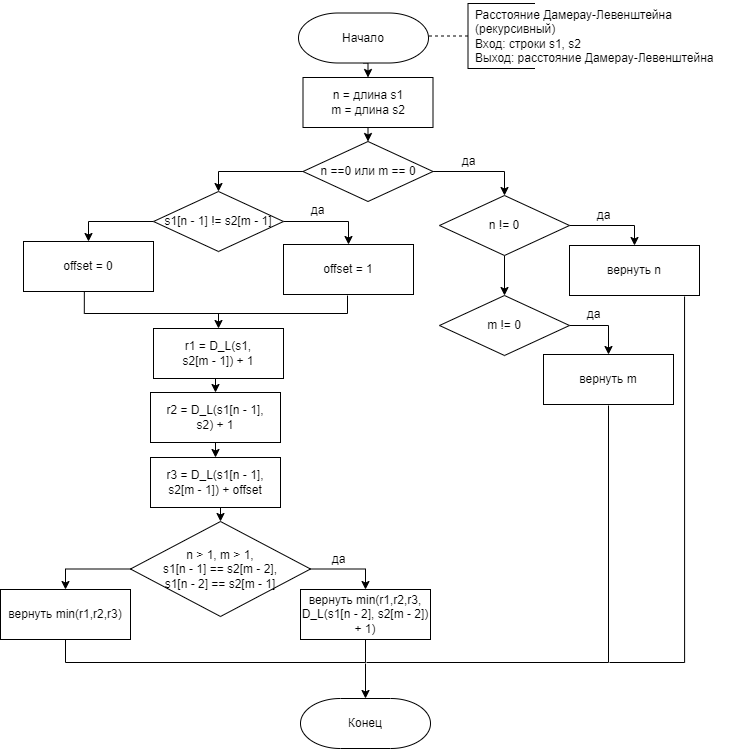
\includegraphics[width=1\linewidth]{DamLevRec}
		\caption{Схема рекурсивного алгоритма поиска расстояния Дамерау-Левенштейна}
		\label{fig:schema_selection}
	\end{figure}
	
	\begin{figure}
		\centering
		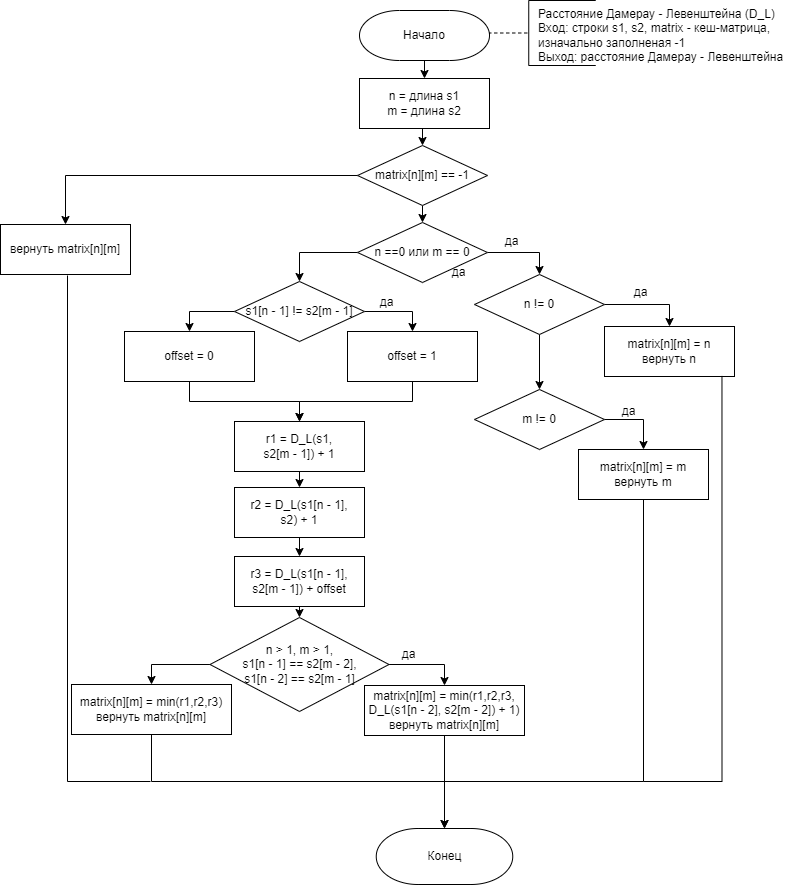
\includegraphics[width=1\linewidth]{DamLevRecCash}
		\caption{Схема рекурсивного алгоритма поиска расстояния Дамерау-Левенштейна с кешем}
		\label{fig:schema_selection}
	\end{figure}

        \clearpage
	\section*{Вывод}
	
	В данном разделе на основе теоретических данных были построены схемы требуемых алгоритмов, выбраны используемые типы данных, а также была проведена оценка затрачиваемого объёма памяти.
	
	\chapter{Технологическая часть}
	
	\section{Требования к программному обеспечению}
	
	В программе должна присутствовать возможность:
	
	\begin{enumerate}
		\item[1)] ввода исходных слов, для которых будут находиться расстояния Левенштейна и Дамерау-Левенштейна;
		\item[2)] поиска искомого расстояния для введеных строк с помощью одного из четырех рассматриваемых алгоритмов;
		\item[3)] замера процессорного времени выполнения реализаций алгоритмов поиска расстояний Левенштейна и Дамерау-Левенштейна.
	\end{enumerate}
	
	\section{Выбор языка программирования}
	
	Для реализации алгоритмов поиска редакционных расстояний был выбран язык программирования С в силу наличия точных библиотек для замеров процессорного времени и быстродейственности языка.
	
	\section{Выбор библиотеки и способа для замера времени}
		Для замера процессорного времени выполнения реализаций агоритмов была выбрана не стандартная функция библиотеки <time.h> языка С~---~clock(), которая недостаточно четко работает при замерах небольших промежутков времени, а QueryPerformanceCounter - API-интерфейс, использующийся для получения меток времени с высоким разрешением или измерения интервалов времени.
        
        Для облегчения работы с данным инструментом были самостоятельно написаны обертки-макросы, представленные на листинге \ref{time}.
        
        \clearpage
        
        \begin{lstlisting}[label= time,caption=Листинг макросов, используемых для замеров процессорного времени,language=C]
    #define TIMER_INIT \
        LARGE_INTEGER frequency; \
        LARGE_INTEGER t1,t2; \
        double elapsedTime; \
        QueryPerformanceFrequency(&frequency);
            
    #define TIMER_START QueryPerformanceCounter(&t1);
            
    #define TIMER_STOP \
        QueryPerformanceCounter(&t2); \
        elapsedTime=(float)(t2.QuadPat1.QuadPart)/frequency.QuadPart/COUNT*MICRO; \
        printf("%lf", elapsedTime);
        \end{lstlisting}
		
	В силу существования явления вытеснения процессов из ядра, квантования процессорного времени все процессорное время не отдается какой-либо одной задаче, поэтому для получения точных результатов необходимо усреднить результаты вычислений: замерить совокупное время выполнения реализации алгоритма N раз и вычислить среднее время выполнения.
		
	\section{Реализации алгоритмов}
	
	В листингах \ref{lev}, \ref{damlev}, \ref{damlevrec}, \ref{damlevrechash} приведены реализации алгоритмов поиска расстояний Левенштейна (итерационный), Дамерау-Левенштейна (итерационный), \mbox{Дамерау-Левенштейна} (рекурсивный), Дамерау-Левенштейна (рекурсивный с кешем) соответсвенно.
	
	\begin{lstlisting}[label=lev,caption=Листинг итерационного алгоритма поиска расстояния Левенштейна,language=C]
    int lev(char *str_1, char *str_2, int print_table_flag)
    {
        matrix_t *m = create_matrix(strlen(str_1) + 1, strlen(str_2) + 1);
    
        m->elements[0][0] = 0;
        for (size_t i = 1; i < m->rows; ++i)
            m->elements[i][0] = i;
        for (size_t i = 1; i < m->cols; ++i)
            m->elements[0][i] = i;
    
        for (size_t i = 1; i < m->rows; ++i)
            for (size_t j = 1; j < m->cols; ++j) 
    		{
                int offset = str_1[i - 1] == str_2[j - 1] ? 0 : 1;
                m->elements[i][j] = min(3, m->elements[i][j - 1] + 1,
                                           m->elements[i - 1][j] + 1,
                                           m->elements[i - 1][j - 1] + offset);
            }
    
        int res = m->elements[m->rows - 1][m->cols - 1];
        free_matrix(m);
    
        return res;
    }
	\end{lstlisting}

	
	\begin{lstlisting}[label=damlev,caption=Листинг итерационного алгоритма поиска расстояния Дамерау-Левенштейна,language=C]
    int dameray_lev(char *str_1, char *str_2, int print_table_flag)
    {
        matrix_t *m = create_matrix(strlen(str_1) + 1, strlen(str_2) + 1);
    
        m->elements[0][0] = 0;
        for (size_t i = 1; i < m->rows; ++i)
            m->elements[i][0] = i;
        for (size_t i = 1; i < m->cols; ++i)
            m->elements[0][i] = i;
    
        for (size_t i = 1; i < m->rows; ++i)
            for (size_t j = 1; j < m->cols; ++j) {
                int offset = str_1[i - 1] == str_2[j - 1] ? 0 : 1;
                m->elements[i][j] = min(3, m->elements[i][j - 1] + 1,
                                           m->elements[i - 1][j] + 1,
                                           m->elements[i - 1][j - 1] + offset);
                if (j > 1 && i > 1 && str_1[i - 1] == str_2[j - 2] && str_1[i - 2] == str_2[j - 1])
                    m->elements[i][j] = min(2, m->elements[i][j], m->elements[i - 2][j - 2] + 1);
            }
    
        int res = m->elements[m->rows - 1][m->cols - 1];
        free_matrix(m);
    
        return res;
    } 
	\end{lstlisting}
	
	\bigbreak

	\begin{lstlisting}[label=damlevrec,caption=Листинг рекурсивного алгоритма поиска расстояния Дамерау-Левенштейна,language=C]
    int dameray_lev_rec(char *str_1, char *str_2, int len_1, int len_2)
    {
        if (len_1 == 0)
            return len_2;
        if (len_2 == 0)
            return len_1;
    
        int offset = str_1[len_1 - 1] == str_2[len_2 - 1] ? 0 : 1;
        int res = min(3, dameray_lev_rec(str_1, str_2, len_1 - 1, len_2)                    + 1,
                         dameray_lev_rec(str_1, str_2, len_1, len_2 - 1) + 1,
                         dameray_lev_rec(str_1, str_2, len_1 - 1, len_2 - 1) + offset);
        if (len_1 > 1 && len_2 > 1 && str_1[len_1 - 1] == str_2[len_2 - 2] && str_1[len_1 - 2] == str_2[len_2 - 1])
            res = min(2, res, dameray_lev_rec(str_1, str_2, len_1 - 2, len_2 - 2) + 1);
    
        return res;
    } 
	\end{lstlisting}
	
	\begin{lstlisting}[label=damlevrechash,caption=Листинг рекурсивного алгоритма поиска расстояния Дамерау-Левенштейна с кешем,language=C]	
    int dameray_lev_rec_cache_call(char *str_1, char *str_2, int len_1, int len_2, matrix_t *mat)
    {
        if (len_1 == 0)
            return (mat->elements)[len_1][len_2] = len_2;
        if (len_2 == 0)
            return (mat->elements)[len_1][len_2] = len_1;
    
        if (mat->elements[len_1 - 1][len_2] == -1)
            dameray_lev_rec_hash_call(str_1, str_2, len_1 - 1, len_2, mat);
        if (mat->elements[len_1][len_2 - 1] == -1)
            dameray_lev_rec_hash_call(str_1, str_2, len_1, len_2 - 1, mat);
        if (mat->elements[len_1 - 1][len_2 - 1] == -1)
            dameray_lev_rec_hash_call(str_1, str_2, len_1 - 1, len_2 - 1, mat);
    
        int offset = str_1[len_1 - 1] == str_2[len_2 - 1] ? 0 : 1;
        mat->elements[len_1][len_2] = min(3, mat->elements[len_1][len_2 - 1] + 1,
    										 mat->elements[len_1 - 1][len_2] + 1,
                                             mat->elements[len_1 - 1][len_2 - 1] + offset);
        if (len_1 > 1 && len_2 > 1 && str_1[len_1 - 1] == str_2[len_2 - 2] && str_1[len_1 - 2] == str_2[len_2 - 1]) {
            if (mat->elements[len_1 - 2][len_2 - 2] == -1)
                dameray_lev_rec_hash_call(str_1, str_2, len_1 - 2, len_2 - 2, mat);
            mat->elements[len_1][len_2] = min(2, mat->elements[len_1][len_2], mat->elements[len_1 - 2][len_2 - 2] + 1);
        }
    
        return mat->elements[len_1][len_2];
    }
    
    int dameray_lev_rec_cache(char *str_1, char *str_2)
    {
        matrix_t *m = create_matrix(strlen(str_1) + 1, strlen(str_2) + 1);
        clear_matrix(m);
    
        int res = dameray_lev_rec_hash_call(str_1, str_2, strlen(str_1), strlen(str_2), m);
        free_matrix(m);
    
        return res;
    } 
	\end{lstlisting}

\section{Тестирование алгоритмов}

В таблице~\ref{tbl:test} приведены проведенные тесты для функций, реализующих алгоритмы поиска расстояний Левенштейна и Дамерау-Левенштейна.
	
\begin{table}[h!]
	\begin{center}
        \captionsetup{justification=raggedright,singlelinecheck=off}
		\caption{\label{tbl:test} Тестирование функций}
		\begin{tabular}{|c|c|c|c|}
			\hline
			Первое слово & Второе слово & Расстояние Лев. & Расстояние Дам.-Лев. \\ 
			\hline
			$\lambda$ & $\lambda$ & $0$ & $0$\\\hline
			$cat$  & $\lambda$ & $3$ & $3$\\\hline
			$cat$  & $cat$  & $0$ & $0$\\\hline
			$cat$  & $catdog$  & $3$ & $3$\\\hline
			$hotdog$ & $hodtog$ & $2$ & $1$\\\hline	
		\end{tabular}			
	\end{center}
\end{table}

\section*{Вывод}
В данном разделе были разработаны алгоритмы поиска расстояний Левенштейна и Дамерау–Левенштейна, а также проведено тестирование.
	
\chapter{Экспериментальная часть}
	
\section{Технические характеристики}
Ниже приведены технические характеристики устройства, на котором было проведено тестирование программного обеспечения:
	
\begin{enumerate}
	\item[1)] операционная система Windows-10, 64-bit;
	\item[2)] оперативная память 8 ГБ;
	\item[3)] процессор	Intel(R) Core(TM) i3-7020U CPU @ 2.30GHz, 2304 МГц, ядер 2, логических процессоров 4.
\end{enumerate}
	
\section{Замеры времени}
	
В таблице \ref{table:t1} приведены результаты замеров в микросекундах времени алгоритмов для входных строк разной длины.
 
	\begin{table} [h!]
        \captionsetup{justification=raggedright,singlelinecheck=off}
		\caption{Таблица замера времени выполнения алгоритмов на строках, имеющих разные длины}
		\label{table:t1}
		\begin{center}
			\begin{tabular}{|c | c | c | c | c|}
				
				\hline
				
				Длина стоки & Лев. & Дам.-Лев. & Дам.-Лев.(рек.) &   Дам.-Лев.(рек. с кэшем)  \\ [0.5ex]
				
				\hline
				
				1 & 1.15 & 1.12 & 0.11 & 0.96 \\ 
				
				\hline 
				
				2 & 1.57 & 1.08 & 0.24 & 1.96 \\ 
				
				\hline 
				
				3 & 2.71 & 2.84 & 1.36 & 1.61 \\ 
				
				\hline 
				
				4 & 1.56 & 2.56 & 6.30 & 3.94 \\ 
				
				\hline 
				
				5 & 2.85 & 3.71 & 44.91 & 4.11 \\ 
				
				\hline 
				
				6 & 5.35 & 6.73 & 161.43 & 5.47 \\ 
				
				\hline 
				
				7 & 6.60 & 7.40 & 1061.13 & 6.12 \\ 
				
				\hline 
				
				8 & 5.43 & 6.27 & 5355.47 & 4.91 \\ 
				
				\hline 
				
				9 & 3.70 & 4.47 & 30525.51 & 8.21\\ 
				
				\hline 
				
				10 & 5.24 & 6.52 & 180535.97 & 6.95\\ 
				
				\hline 
			\end{tabular}
		\end{center}
	\end{table}

	Зависимость времени работы алгоритмов поиска расстояний Левенштейна (итерационный), Дамерау-Левенштейна (итерационный), Дамерау-Левенштейна (рекурсивный с кешем) от длины входных строк представлена на рисунке \ref{ris1}.

	\begin{center}
		\begin{figure}[h!]
		\center
		\begin{tikzpicture}
				\begin{axis} [
					legend pos = north west,
					grid = major,
					xmin = 0,
					ymin = 0, 
					xmax = 10,
					ymax = 15,
					xlabel = $\text{длина входных строк в символах}$,
					ylabel = $\text{время в мс}$
					]
					\legend{ 
						$Lev$, 
						$DamLev$,
						$DamLevRec$,
						$DamLevRecCache$
					};
					\addplot coordinates {
						(1, 1.15) (2, 1.57) (3, 2.71) (4, 1.56) (5, 2.85) (6, 5.35) (7, 6.60) (8, 5.43) (9, 3.70) (10, 5.24)
					};
					\addplot coordinates {
						(1, 1.12) (2, 1.08) (3, 2.84) (4, 2.56) (5, 3.71) (6, 6.73) (7, 7.40) (8, 6.27) (9, 4.47) (10, 6.52)
					};
					\addplot coordinates {
						(1, 0.96) (2, 1.96) (3, 1.61) (4, 3.94) (5, 4.11) (6, 5.47) (7, 6.12) (8, 4.91) (9, 8.21) (10, 6.95)
					};
				\end{axis}
		\end{tikzpicture}
		  \caption{Зависимость времени от длины входных строк}
		\label{ris1}
		\end{figure}
	\end{center}
	
	
	Зависимость времени работы алгоритма поиска расстояний Дамерау-Левен\-штейна (рекурсивный) от длины входных строк представлена на рисунке \ref{ris2}.


	\begin{center}
		\begin{figure}[h!]
		\center
		\begin{tikzpicture}
			\begin{axis} [
				legend pos = north west,
				grid = major,
				xmin = 0,
				ymin = 0, 
				xmax = 10,
				ymax = 190000,
				xlabel = $\text{длина входных строк в символах}$,
				ylabel = $\text{время в мс}$
				]
				\legend{ 
					$DamLevRec$,
				};
				\addplot coordinates {
					(1, 0.11) (2,0.24) (3, 1.36) (4, 6.30) (5, 44.91) (6, 161.43) (7, 1061.13) (8, 5355.47) (9, 30525.51) (10, 180535.97)
				};
			\end{axis}
		\end{tikzpicture}
		\caption{Зависимость времени от длины входных строк}
		\label{ris2}
		\end{figure}
	\end{center}

	\section*{Вывод}
	
	Результаты замеров показали, что рекурсивный алгоритм поиска расстояния Дамерау-Левенштейна работает дольше всего. 
    При этом его оптимизация с кешем работает в разы быстрее. 
    Итерационные алгоритмы нахождения расстояний Левенштейна и Дамерау-Левенштейна оказались наиболее быстрыми, причем на длине строки от 1 до 10 элементов итерационный алгоритм Левенштейна в среднем работает немного быстрее, нежели итерационный алгоритм нахождения расстояния Дамера-Левенштейна. 
	
\chapter*{Заключение}
	
Цель лабораторной работы достигнута -- были получены навыки динамического программирования на примере разработки алгоритмов поиска редакционных расстояний. Все задачи решены:
	
	\begin{enumerate}
		\item[1)] изучены расстояния Левенштейна и Дамерау-Левенштейна;
		\item[2)] разработаны указнные алгоритмы поиска расстояний;
		\item[3)] реализованы разработанные алгоритмы;
		\item[4)] была рассчитана их трудоемкость по памяти;
		\item[5)] проведен сравнительный анализ реализаций алгоритмов по затраченному процессорному времени и памяти на основе экспериментальных данных;
		\item[6)] описаны и обоснованы полученные результаты в отчете о выполненной лабораторной работе.
	\end{enumerate}
	
	На основании проведенных экспериментов было определено, что время работы алгоритмов с увелечением длины строк увеличивается в геометрической прогрессии. 
    Самым медленным по скорости выполнения, но наименне затратным по памяти оказался рекурсивный алгоритм определения расстояния Дамерау-Левенштейна.
    Самым быстрым же оказался итерационный алгоритм нахождения расстояния Левенштейна, который одновременно с этим, оказался одним из самых затратных по памяти, так как в его реализации дополнительно используется матрица, размером, соответсвующим длине входных строк.
	
\addcontentsline{toc}{chapter}{Список использованных источников}

\nocite{*} 

\renewcommand\bibname{Список использованных источников} % переименовать страницу списка литературы
\bibliographystyle{utf8gost705u}  % стилевой файл для оформления по ГОСТу
\bibliography{lib}          % имя библиографической базы (bib-файла)
	
\end{document}
